\documentclass[a4paper, 12pt]{scrartcl}

%===============================================================================
% Packages
%===============================================================================
\usepackage{fontspec}
\usepackage{geometry}
\usepackage[ngerman]{babel} % Use new german language definition
\usepackage{hyperref} % Hyperlinks in PDFs
\usepackage{amsmath, amsfonts, amssymb} % Math packages
\usepackage{graphicx} % For Graphics
\usepackage{xcolor} % For coloring texts
\usepackage{times} % Times New Roman Font
\usepackage{tikz} % The TikZ vector graphic library
\usepackage{fancyhdr} % Fancy headings
\usepackage{nameref} % References for names instead of numbers
\usepackage[absolute]{textpos} % Absolute positioning
\usepackage{titlesec} % Customizable ((Sub)Sub)Sections
\usepackage[titles]{tocloft} % Customizable ToC, LoF, …
\usepackage{pdfpages} % Embedding pdfs
\usepackage{wallpaper} % Background images
\usepackage{tikz-er2} % Entity relation diagrams
\usepackage{listings} % Code listings
\usepackage{acronym} % Using acronyms
\usepackage{natbib} % Literature

%===============================================================================
% Tikz-Librarys
%===============================================================================
\usetikzlibrary{positioning}
\usetikzlibrary{shadows}

\tikzstyle{every node} = [font=\sffamily]
\tikzstyle{every entity} = [top color=kiba!10, bottom color=kiba!70, 
                            draw=kiba!80!black, drop shadow, font=\sffamily\bfseries]
\tikzstyle{every weak entity} = [drop shadow={shadow xshift=.7ex, 
                                 shadow yshift=-.7ex}]
\tikzstyle{every attribute} = [top color=white, bottom color=black!10, 
                               draw=black!50, node distance=1cm, drop shadow]
\tikzstyle{every relationship} = [top color=white, bottom color=red!20, 
                                  draw=red!50!black!100, drop shadow, font=\sffamily\itshape]
\tikzstyle{cty} = [auto, font=\sffamily\footnotesize]
\tikzstyle{every isa} = [top color=white, bottom color=green!20, 
                         draw=green!50!black!100, drop shadow]
                         
%===============================================================================
% BibTeX
%===============================================================================
\makeatletter
\newcommand{\bibstyle@dinat}%
	{\bibpunct{(}{)}{;}{a}{}{,~}%
		\gdef\NAT@biblabelnum##1{\textbf{##1}}}
\makeatother
                         
%===============================================================================
% Listings
%===============================================================================
\lstset{
	emph={KBABranchDao, KBAAccountDao, KBACustomerDao, KBATransactionDao, KBAExchangeRateDao, KBACustomerDao, KBACreditRatingDao, KBAMessageDao, KBAAuth, KBADependencyInjector, KibaTests, KBABootstrap},
	emph={[2]NSString, XCTAssert},
	language=[Objective]C, 
	morekeywords={new,@,},
	backgroundcolor=\color{black!3},
	columns=fullflexible,
	basicstyle=\ttfamily\footnotesize,
	keywordstyle=\bfseries\ttfamily\color{blue!50!red!80!black},
	stringstyle=\color{red!70!black}\ttfamily,
	identifierstyle=\ttfamily\itshape,
	commentstyle=\color{green!30!black}\ttfamily\itshape,
	emphstyle={\color{orange!70!black}\bfseries\texttt},
	emphstyle={[2]\color{green!60!blue!50!black}\bfseries\texttt},
	showstringspaces=false,
	flexiblecolumns=false,
	tabsize=4,
	lineskip={-1pt}
}
\makeatletter
\begingroup\let\newcounter\@gobble\let\setcounter\@gobbletwo
  \globaldefs\@ne \let\c@loldepth\@ne
  \newlistof{listings}{lol}{\lstlistlistingname}
\endgroup
\let\l@lstlisting\l@listings
\AtBeginDocument{\addtocontents{lol}{\protect\addvspace{10\p@}}}
\makeatother
\renewcommand{\lstlistoflistings}{\listoflistings}

%===============================================================================
% Definitions
%===============================================================================
%\newcommand{\semantischerAusdruck}[1]{%
%	... was macht das ... #1

\newcommand{\Stichwort}[1]{%
	\textbf{#1}}
\setlength{\parskip}{6pt}
\renewcommand{\headrulewidth}{0pt}
\linespread{1.5}
\geometry{a4paper}
\geometry{left=25mm,right=25mm,bottom=30mm,top=30mm}
\geometry{footnotesep=5mm}
\geometry{headsep=10mm}
\geometry{head=10mm}
\geometry{bindingoffset=0mm}
\definecolor{kiba}{HTML}{41707C}
\newcommand{\pre}[1]{%
	\texttt{#1}}
\renewcommand\UrlFont{}

%===============================================================================
% Collaborative
%===============================================================================
\definecolor{markus}{HTML}{FF3118}
\definecolor{alex}{HTML}{3152A5}
\definecolor{julius}{HTML}{639C18}
\definecolor{marco}{HTML}{844D18}
\definecolor{michael}{HTML}{A50063}
\definecolor{corny}{HTML}{0084A5}

\makeatletter
\def\name@markus{Markus Fasselt}
\def\name@alex{Alexander Droste}
\def\name@julius{Julius Wulk}
\def\name@marco{Marco F. Jendryczko}
\def\name@michael{Michael Schaarschmidt}
\def\name@corny{Konstantin S. M. Möllers}
\newcommand{\currentAuthor}{kiba}
\newcommand{\authoredSection}[2]{%
	\renewcommand{\currentAuthor}{#1}%
	\pagebreak
	\section[#2]{#2 {\normalfont\sffamily\small von \csname name@#1\endcsname}}}
\makeatother
\renewcommand{\lstlistingname}{Programmausdruck}
\renewcommand{\lstlistlistingname}{Programmausdrucksverzeichnis}

%===============================================================================
% Head / Foot
%===============================================================================
\pagestyle{fancy}
\fancyhf{}
\makeatletter
\fancyhead[L]{}
\fancyhead[R]{\sffamily\itshape Projektbericht „KiBa“-App}
\fancyfoot[C]{}
\fancyfoot[R]{\sffamily\thepage}
\makeatother

%===============================================================================
% Font
%===============================================================================
\setmainfont{TeX Gyre Termes}
\setsansfont[
	Extension = .ttf,
	Path = Fonts/,
	BoldFont = TheSansUHHBold,
	BoldItalicFont = TheSansUHHBolditalic,
	ItalicFont = TheSansUHHRegularItalic
]{TheSansUHHRegular}
\setmonofont[
	Extension = .otf,
	Path = Fonts/,
	BoldFont = lmmonolt10-bold,
	BoldItalicFont = lmmonolt10-boldoblique,
	ItalicFont = lmmonolt10-oblique
]{lmmono12-regular}
\defaultfontfeatures{Ligatures=TeX}

%===============================================================================
% Sections
%===============================================================================
\titleformat{\section}[hang]{\Large\sffamily\bfseries\color{\currentAuthor}}{\thesection\quad}{0pt}{}
\titleformat{\subsection}[hang]{\large\sffamily\itshape}{\thesubsection\quad}{0pt}{}
\titleformat{\subsubsection}[hang]{\large\sffamily}{\thesubsubsection\quad}{0pt}{}

%===============================================================================
% Table of Contents
%===============================================================================
\renewcommand{\cftdotsep}{\cftnodots}
\renewcommand{\cftsecfont}{\bfseries\sffamily}
\renewcommand{\cftfigpresnum}{Abb. }
\renewcommand{\cfttabpresnum}{Tab. }
\renewcommand{\cftlistingspresnum}{Prog. }
\renewcommand{\cftfigaftersnum}{:}
\renewcommand{\cfttabaftersnum}{:}
\renewcommand{\cftlistingsaftersnum}{:}
\setlength{\cftfignumwidth}{2cm}
\setlength{\cfttabnumwidth}{2cm}
\setlength{\cftlistingsnumwidth}{2cm}
\setlength{\cftfigindent}{0cm}
\setlength{\cfttabindent}{0cm}
\setlength{\cftbeforelistingsskip}{-2mm}
\setlength{\cftlistingsindent}{0cm}
\setlength{\cftbeforesubsecskip}{-1mm}
\setlength{\cftbeforesubsubsecskip}{-1mm}
\setlength{\cftsubsecindent}{0cm}
\setlength{\cftsubsubsecindent}{0cm}
\def\tocnumwidth{13mm}
\setlength{\cftsecnumwidth}{\tocnumwidth}
\setlength{\cftsubsecnumwidth}{\tocnumwidth}
\setlength{\cftsubsubsecnumwidth}{\tocnumwidth}
    
%===============================================================================
% Meta Description
%===============================================================================    
\author{%
	Alexander Droste\vphantom{yMö}\\[-2pt]
    Markus Fasselt\vphantom{yöM}\\[-2pt]
    Marco F. Jendryczko\vphantom{yMö}\\[-2pt]
    Konstantin S. M. Möllers \vphantom{yMö}\\[-2pt]
    Michael Schaarschmidt\vphantom{yöM}\\[-2pt]
    Julius Wulk\vphantom{yMö}}
\title{Die „KiBa“-App}
\date{Wintersemester 2013/14}
\hypersetup{pdftitle = {Die \glqq{}KiBa\grqq{}-App},
            pdfsubject = {Projektbericht der App},
            pdfauthor = {Droste, Fasselt, Jendryczko, M\"ollers, Schaarschmidt, Wulk},
            pdfcreator = {Gruppe 1 - KiBa},
            pdfproducer = {KiBa App PDF},
            linkbordercolor = {.25390625 .4375 .484375},
            urlbordercolor = {.25390625 .4375 .484375}}

    
%===============================================================================
% Document
%===============================================================================
\begin{document}
	
\makeatletter
\thispagestyle{empty}

\begin{center}
	\textcolor{kiba}{\bf\sffamily\fontsize{48pt}{48pt}\selectfont \@title} \\[.5cm]
	\includegraphics[height=3cm]{logo-kiba} \\[.5cm]
	\textcolor{kiba}{\LARGE\sffamily Projektbericht} \\[.5cm]
    {\large\sffamily Angefertigt von} \\[4pt]
    {\Large \@author \\[1.5cm]}
    {\large\sffamily Veranstalter} \\[12pt]
    {\Large Dr. Guido Gryczan} \\[6pt] {\LARGE Dr. Martin Christof Kindsmüller\vphantom{y}} \\[6pt] {\LARGE Christian Zoller} \\[1.5cm]
    {\Large\sffamily \@date}
\end{center}

\vspace{2.5cm}

% UHH-Logo
\begin{textblock*}{85mm}(20mm, 257mm)
	\includegraphics[width=2cm]{logo-uhh}\;{\sffamily Universität Hamburg}
\end{textblock*}

% FBI-Logo
\begin{textblock*}{85mm}(105mm, 257mm)
	\hfill{\sffamily Fachbereich Informatik}\;\includegraphics[width=2cm]{logo-fbi}
\end{textblock*}

\makeatother
\newpage
    
\tableofcontents
\newpage

%===============================================================================
% Listings
%===============================================================================
\phantomsection
\addcontentsline{toc}{section}{\lstlistlistingname}
\lstlistoflistings

%===============================================================================
% Acronyms
%===============================================================================
\section*{Abkürzungsverzeichnis}
\phantomsection
\addcontentsline{toc}{section}{Abkürzungsverzeichnis}
\begin{acronym}[SOAP]
	\acro{DAO}{Data Access Object}
	\acro{REST}{Representational State Transfer}
	\acro{SOAP}{Simple Object Access Protocol}
	\acro{VCS}{Version Control System (Versionsverwaltung)}
\end{acronym}
\newpage

%===============================================================================
% Parts
%===============================================================================
\authoredSection{michael}{Einleitung und Projektkontext}
	Der vorliegende Bericht soll die rückblickende Betrachtung eines universitären Software-Pro\-jekts konstituieren, bei dem über ein Semester hinweg in Kooperation mit der T-Systems MMS eine iOS-Anwendung entwickelt wurde. Die zentrale Herausforderung war dabei, universitäre Erfordernisse mit kommerziellen Anforderungen in Einklang zu bringen. Ziel war es, anhand einer gegebenen Aufgabenstellung in Gruppen mit universitär heterogenem Hintergrund einen Prototypen zu entwickeln.
	
	Dieser sollte in Architektur und Gestaltung das Verständnis softwaretechnischer und interaktiver Konzepte deutlich machen, gleichzeitig aber geeignet sein, in einer konkreten Produktdemonstration im Projektabschluss praktischen Nutzen unter Beweis zu stellen. Zusätzlich wurden wir im Rahmen einer in das Projekt integrierten, einführenden Zertifizierung mit der Scrum-Methodik vertraut gemacht, welche dann als Grundlage für die Projektarbeit diente. 

	Die unser Gruppe übertragene Aufgabe bestand darin, eine App zu entwickeln, welche die Bindung zwischen einer fiktiven Filialbank und ihren Kunden erhöht. In den ersten Überlegungen wurde deutlich, dass nahezu jede Dienstleistung einer Filiale auf die eine oder andere Weise von Direktbanken abgebildet werden kann. Nicht umsonst ist das Filialgeschäft im Abschwung \footnote{\url{http://www.welt.de/print/wams/wirtschaft/article124228415/Das-ist-ein-Sterben-auf-Raten.html}, \\Abruf am 23.02.2014 um 16:00 Uhr.}. Es erscheint insofern zunächst widersinnig, ein Geschäftsmodell, welches zunehmend effizient durch Softwareprodukte ersetzt wird und nur noch wenig profitabel ist, um jeden Preis erhalten zu wollen. Während nämlich auch im Bankgeschäft parallel zu sozialen Netzwerken Social-Banking-Konzepte erste Anwendung finden \footnote{\url{http://www.visiblebanking.com/commbank-launches-first-social-banking-app-facebook-p2p-payments-7693/},\\ Abruf am 23.02.2014 um 16:05 Uhr.}, haben diese nicht unmittelbar Bezug zum Filialgeschäft.
	 
	Hier wurde uns bewusst, dass als Entwickler in Auftragsarbeit die eigenen Überlegungen hinsichtlich der Entwicklung eines Geschäftsfeldes oder Produktes zurückstehen müssen; vielmehr müssen in einem schwierigen Markt Möglichkeiten gefunden werden, innerhalb der vorhandenen Strukturen zu innovieren.
	 
\authoredSection{michael}{App-Idee}

\subsection{Problematik}
Mit Rücksicht auf oben genannte Aspekte haben wir in der Ideenfindungsphase auf Lokalität als entscheidendes Schlagwort konzentriert. Apps wie etwa foursquare (Quelle?), welche Bezug auf lokale Unternehmen nehmen und Benutzern die Möglichkeit geben, sich darüber auszutauschen, sind beispielhaft für die erfolgreiche Umsetzung dieses Konzepts. Für das Bankgeschäft ergab sich jedoch das Problem, dass die eigenen finanziellen Verhältnisse in den innersten persönlichen Lebensbereich fallen und in der Regel darüber zumindest weniger Austausch stattfindet als über Restaurants, Nachtclubs oder Freizeitaktivitäten. So erschien es uns nachvollziehbar, dass die App eine Interaktion zwischen einem Kunden und einer Filiale begünstigen soll, nicht aber den Austausch zwischen mehreren Kunden - der dann ohnehin wieder kaum eine Filiale benötigen würde.

Erste Überlegungen zielten in Richtung interaktiver Hilfedienstleistungen, welche jederzeit über Videotelefonie Kontakt zum individuell vertrauten Berater einer bestimmten Filiale herstellen sollten. In den wöchentlichen Diskussionen im Projektplenum wurden uns aber Mängel aufgezeigt; der individuelle Berater ist kein Alleinstellungsmerkmal der Filialbank mehr, eine virtuelle Filiale ist ohne weiteres denkbar.

Allerdings, und hier haben wir die Chance unserer App gesehen, heißt die technische Möglichkeit eines Vertriebsweges nicht gleich, dass dieser auch angenommen wird. Eine von uns im Sinne einer Markterkundung durchgeführte Umfrage ergab ein gewisses Misstrauen gegenüber der Idee, Finanztransaktionen per App durchzuführen. Gründe hierfür könnten vielfältig sein, beispielsweise könnten die befragten Studenten am Informatikcampus eine besondere Sensibilität bezüglich Aspekten des Datenschutzes und der Transaktionssicherheit haben. Eine von der Unternehmensberatung Bain and Company durchgeführte Studie zur Frage, wie digitalisierte Vertriebswege das Retailbanking zukünftigen prägen könnten, ergab einen ähnlichen Tenor.
%(http://www.bain.de/Images/Retail_Banking_II_Digitalisierung_ES.pdf).

 Insbesondere ergab die Studie, dass für Geldanlagen dem persönlichen Gespräch der Vorzug gegeben würde. Inwiefern eine solche Studie aussagekräftig für eine Banking-App der Zukunft ist, sei dahingestellt. Schließlich wäre es auch möglich, dass hier einfach noch keine Gewöhnung stattgefunden hat und die Studie nur einen Übergangseffekt widerspiegelt, der für eine langfristig strategische Ausrichtung irrelevant wäre.

\subsection{Vision}


Insofern haben wir uns nach einem Prozess von abwechselnden Gruppendiskussion und externen Feedback dazu entschlossen, diejenigen Features zu betonen, die Berater und Kunden möglichst in der Filiale zusammenbringen, aber auch unabhängig davon genutzt werden können. Auch Direktbanken versuchen inzwischen, anonyme Hotlines zu vermeiden und Kunden einzelnen Beratern zuzuordnen. In Kombination mit niedrigeren Gebühren, kostenlosen Kreditkarten und einfacher Kontoführung ist dies ein schwer zu schlagendes Angebot. Eine App, die Neukunden für eine Filalbank gewinnen soll, muss also einerseits eine ähnlich einfache Kontoverwaltung bieten, außerdem aber noch einen Mehrwert schaffen, der die höheren Gebühren einer Filialbank rechtfertigt.

Ein weiterer, für die Akzeptanz einer App wichtiger Aspekt ist die (vielleicht auch nur vom Kunden gefühlte) Sicherheit. Eine von uns durchgeführte Umfrage unter Studenten technischer Fächer, primär Informatik, ergab, dass die meisten Teilnehmer unabhängig von der Funktionalität schon aus Sicherheitsgründen keine Bankgeschäfte mit einer App erledigen wollten. Die besondere Sensibilität der genannten Zielgruppe für Sicherheitsaspekte darf nicht außer Acht gelassen werden; dennoch ergab sich für uns die Frage, ob hier durch Interaktion in der Filiale nicht zugleich Kundenbindung und Vertrauen in die Sicherheit der Anwendung erhöht werden könnten. 

Insgesamt entstand also die Vorstellung einer Anwendung, die klassische Bankgeschäfte wie Überweisungen beherrscht, gleichzeitig aber versucht, Lokalität und Interaktion mit dem eigenen Berater herzustellen. 

\subsection{Name}
    Der Name der App, "`\textbf{K}i\textbf{B}a"', steht in Anlehnung an eine bekannte Direktbank für eine kundeninteressierte Bank, die mit der Anwendung mehr über ihre Kunden erfahren möchte und mit ihnen in Austausch treten will, um spezifischere Angebote und Beratungen anbieten zu können.
    
\subsection{Gerät}
    Bei der Erstellung eines konkreten Konzepts der Funktionalität haben wir zunächst die Anwendungsfälle besprochen, um die Gerätfrage zu klären. Zweifelsohne gibt es Features, die in einem mobilen Anwendungsfall wahrscheinlicher sind, etwa das Auffinden einer Filiale oder eines Geldautomaten. Eine solche Funktionalität wäre aber nicht filialbankspezifisch. Überhaupt erschien es uns, als wäre der typische Anwendungsfall eher stationär, auf dem Sofa, im Büro, jedenfalls aber in Ruhe. Ein überzeugendes Argument für eine iPad-App ist auch, dass Kunde und Berater in der Filiale zusammen mit der App interagieren und Dinge visualisieren können. Die Vorstellung, ein Kreditangebot auf dem Bildschirm eines iPhones durchzusprechen, ist hingegen eher absurd. 
    
    
    Somit überwogen in der Gruppe ganz eindeutig die Argumente für eine iPad-Anwendung. Zudem war es Aufgabe, eine Vision für die Banking-App der Zukunft zu entwickeln. Der Trend geht unserer Meinung nach zum ubiquitären W-Lan; so gibt es beispielsweise Bestrebungen, öffentliche Netzwerke in der Innenstadt einzurichten. Insofern darf davon ausgegangen werden, dass die mobile Konnektivität zukünftig auch beim iPad zukünftig unproblematisch ist und somit webbasierte Funktionalität auch unterwegs gegeben ist.
    

\subsection{Funktionen}
    Die Kernfunktionen der App sollen sich auf genau die Bereiche konzentrieren, die einer Direktbank nicht zur Verfügung stehen und somit nicht trivial nachgebaut werden können. Dabei haben wir im Zuge der Plenumsdiskussionen und anschließenden internen Debatten insbesondere den zeitlichen Aspekt als zentrale Komponente identifziert. Viele Bescheinigungen und Unterlagen im täglichen Leben werden auch heute noch konkret ausgedruckt benötigt. Der typische Ablauf einer Direktbank sieht so aus, eine Anfrage (etwa nach Wertpapierzweitschriften) per Kontaktformular abzuschicken und dann einige Tage auf die entsprechenden Ausdrucke zu warten. Unsere Idee besteht in einer Self-Service Station innerhalb der Bank, die das Konzept bestehender Automaten erweitert. Ein Kunde kann sein Ipad auf eine Ablage legen und sich mit der Station verbinden. Die Station beinhaltet einen Multifunktionsdrucker und per App können verschiedenste Bescheinigungen ausgedruckt werden. 
    
    Ein wesentliches Produkt von Filialbanken ist das klassische Sparbuch. Umbuchungen können üblicherweise nur in einer Filiale vorgenommen werden, überwiesen werden kann nur auf das Sparkonto. Die Greifbarkeit des Sparbuches vermittelt konservativen, besorgten Sparern ein Gefühl von Sicherheit. Gleichzeitig kann es aber durch diese funktionale Einschränkung auch zu unerwünschten Situationen kommen: ist etwa durch eine Fehlkalkulation an einem Samstagabend kein Geld mehr auf dem Girokonto, muss bis zur Öffnung einer Filiale am Montag gewartet werden, um Guthaben umbuchen zu können. Um dem Vorzubeugen, soll über die Self-Service Station auch Geld umgebucht werden können. Da die Station im Vorraum der Filiale steht, ist sie ganztägig zugänglich. Auf diese Weise bleibt einerseits das Sparbuch als vertrauenswürdige Marke erhalten, die in der Wahrnehmung misstrauischer Benutzer von den Verwerfungen der Online-Kriminalität unberührt bleibt, andererseits ist die Verfügbarkeit erheblich verbessert.
    
    Ebenfalls auf die Bereitstellung von Service-Dienstleistungen zielt der interaktive Filialfinder ab. Aus der Karte heraus sollen Anfragen an eine bestimmte Filiale in der Umgebung er möglicht werden, indem etwa ein Beratungstermin reserviert wird und dann ohne Anstehen erfolgen kann. Eine Funktionalität dieser Art ist 
      
    Als Startbildschirm für die App ist ein Dashboard vorgesehen, das einen graphischen Überblick über Vermögensverlauf und Transaktionen bereitstellt. Hilfreich war hier die Überlegung, dass die meisten Benutzer ihren Kontostand grob kennen und weniger an einer Zahl als vielmehr an den Entwicklungen interessiert sind. Ist der Benutzer nicht eingeloggt, erscheint an dieser Stelle ein Mockup mit der Aufforderung, sich einzuloggen.
    
    Das Kerngeschäft von Filialbanken besteht in der Finanzierung, etwa für Eigenheime. Im Zentrum unserer Überlegungen stand dann auch die Frage, wie eine App dabei helfen kann, diese Dienstleistung für den Endkunden zu verbessern. Im Ergebnis möhten wir einen individualisierten Kreditrechner anbieten, der den App-Benutzer in die Lage versetzt, mittels individuell berechneter Profildaten für sich selbst Finanzierungsrechnungen durchzuführen. Die Idee dahinter ist, dass ein Kunde zunächst für sich selbst einige Finanzierungsvarianten durchspielen kann. Hat er sich eine Variante überlegt, kann ein Termin mit dem persönlichen Berater vereinbart werden und dabei optional gleich der Finanzierungsvorschlag exportiert werden. Im Filialgespräch kann der Berater dann noch individuelle Ratschläge bezüglich Laufzeit und Umfang einer Finanzierung geben.
    
	Eng zusammenhängend mit dem Finanzierungsprofil steht die Aktivierung ("`Authentifikation"') der App in einer Filiale. Ohne eine solche Aktivierung steht dem Benutzer nur passive Funktionalität zur Verfügung, also etwa der Filialfinder und die Umsatzanzeige. Um die App voll nutzen zu können, muss der Benutzer in eine KiBa-Filiale und von einem Berater einen Sicherheitscode eingeben lassen. Ähnlich einer Kreditkarte soll dann bei Gerätverlust auch die App selbst jederzeit gesperrt werden können. Insbesondere dient die Aktivierung aber auch dazu, den Kunden in einem Beratungsgespräch besser kennenzulernen und in einer bankseitigen Datenbank einen persönlichen Ansprechpartner festzuhalten. Aus der App kann dann direkt ein Termin mit dem eingetragenen Berater vereinbart werden. Auch ein Nachrichten-System ist denkbar, um einzelne Fragen direkt zu klären.
\authoredSection{julius}{Kontexterkundung}
Im Rahmen der oben beschriebenen Überlegungen wurde bereits angesprochen, dass wir eine Markterkundung durchgeführt haben. Deren Umsetzung soll hier noch einmal im Detail erläutert werden, um daraus Spezifizierungen für die Mockups zu identifizieren.

\subsection{Fragebogen}
	Bei der Datenerhebung haben wir uns, wie in Abbildung \ref{fig:Questionnaire} zu sehen, für eine Umfrage mittels Fragebogen entschieden, da die App in vielen verschiedenen Kontexten eingesetzt werden soll und wir möglichst viele Meinungen einfließen lassen wollten. 
	
	Für unser Konzept wollten wir wissen, welche Funktionen besonders beliebt sind und welche Bedenken die Teilnehmer bei der Benutzung von Banking-Apps haben. Außerdem war es uns ein Anliegen, nicht nur quantitative, sondern auch qualitative Daten zu erheben. Daher gab es Freitextfelder, in denen die Teilnehmer Ideen, Kritik und allgemeine Bedenken in Bezug auf Banking-Apps äußern konnten. Dieses half uns, die potentiellen Nutzer besser zu verstehen und Dinge aufzudecken, an die wir nicht gedacht hätten. An der Umfrage am Informatikum haben 92 Studenten teilgenommen. Hier folgen nun die wichtigsten Ergebnisse. 
	
\begin{figure}
	\centering
	\begin{tabular}{@{}cc@{}}
		\includegraphics[page=1, scale=.3]{Pictures/Questionnaire} &
		\includegraphics[page=2, scale=.3]{Pictures/Questionnaire}
	\end{tabular}
	\caption{Endfassung des Umfragebogens \label{fig:Questionnaire}}
\end{figure}	
	
\subsection{Ergebnisse}
	Die drei nützlichsten Features sind der Bankautomatenfinder, Filialenfinder und die Kartensperre. Der Bankautmatenfinder wurde von 93\% der Befragten als nützlich bewertet. Das sehr ähnliche Feature Filialenfinder fanden 81\% nützlich und die Kartensperre wurde von 61\% als nützlich angesehen. Diese Ergebnisse zeigen, dass wir die Kernfeatures einer Banking-App nicht aus den Augen verlieren dürfen und dass ein optimierter Finder Potential hat.
	
	48\% der befragten Studenten hielten die Features „Depot-Verwaltung für Aktien“ und „Personalisierte Angebote der Bank“ für nicht nützlich. Eine mögliche Erklärung dafür ist, dass die Studenten bei diesen Themen einfach noch keine eigene Relevanz sehen. 
	
	Ein überraschendes Ergebnis der Umfrage war, dass nur 17\% der befragten Studenten eine Banking App nutzen. Für uns ist es natürlich interessant, aus welchen Gründen Banking-Apps gemieden werden. Studenten gaben an, dass „Apps zu unsicher“ wären, „Apple, Microsoft und Co. Zugriff auf meine Daten“ nähmen, „Unsicherheit der Datenübertragung“, „Bankgeschäfte sollte man in Ruhe bearbeiten und nicht hektisch to go“.
	
	In allen abgefragten Kategorien hatte mindestens über die Hälfte der Studenten Bedenken. Fast 80\% der befragten Studenten gaben an, Angst vor Missbrauch der Daten zu haben. Das zeigt, dass das Thema Sicherheit der eigenen Daten beim Banking eine Schlüsselrolle spielt und wir beim Konzept diesem Aspekt eine besondere Bedeutung zukommen lassen sollten.
	
	Abschließend wollen wir die Ergebnisse in Form eines Diagramms (Abbildung \ref{fig:Kontexterkundung}) präsentieren.
	
\begin{figure}[p]
	\centering
	\includegraphics[scale=.69]{Pictures/Kontexterkundung}
	\caption{Ergebnisse der Kontexterkundung \label{fig:Kontexterkundung}}
\end{figure}
\authoredSection{julius}{User-Interface \& User-Experience}

\subsection{Mockups}
	Vor Beginn der Gestaltung der Mockups haben wir uns auf dem Markt der Banking-Apps umgeschaut, um die verschiedenen UI-Patterns, die in diesem Zusammenhang genutzt werden, zu vergleichen. Mit Balsamiq entwarfen wir anschließend erste Mockups. Bei der Anordnung der Elemente haben wir uns die Prinzipien der Gestaltungsgesetze zunutze gemacht. Insbesondere halfen uns das Gesetz der Ähnlichkeit und das Gesetz der Nähe, Ordnung in die UI zu bringen. 

	Unser Ziel war es, ein möglichst gebrauchstaugliches Design zu erreichen. Dazu haben wir uns an den Grundsätzen der Dialoggestaltung nach der DIN EN ISO 9241 110 orientiert. Bei der Gestaltung haben wir nur eine Schriftart verwendet und uns nach festgelegte Farbsemantiken gerichtet. Dadurch geht der Fokus auf den Inhalt nicht verloren und der Nutzer kann die App erwartungskonform nutzen. Bei der Navigation haben wir uns für eine Master-Detail-View entschieden. Dadurch haben wir eine flache Informationsstruktur, die es uns ermöglicht, alle wichtigen Funktionen von der Hauptseite direkt zu erreichen. Auf diese Weise haben wir unnötige Interaktionen minimiert und der Nutzer kann effizient und aufgabenangemessen mit der App interagieren.  

	Auf jeder Detail-View befindet sich unten rechts ein Informationbutton. Mit diesem Button wollen wir die Selbstbeschreibungsfähigkeit der App verbessern und die Nutzer bei Problemen unterstützen.
	
\begin{figure}[p]
	\centering
	\includegraphics[scale=.52]{Pictures/MockupDashboard}\\
	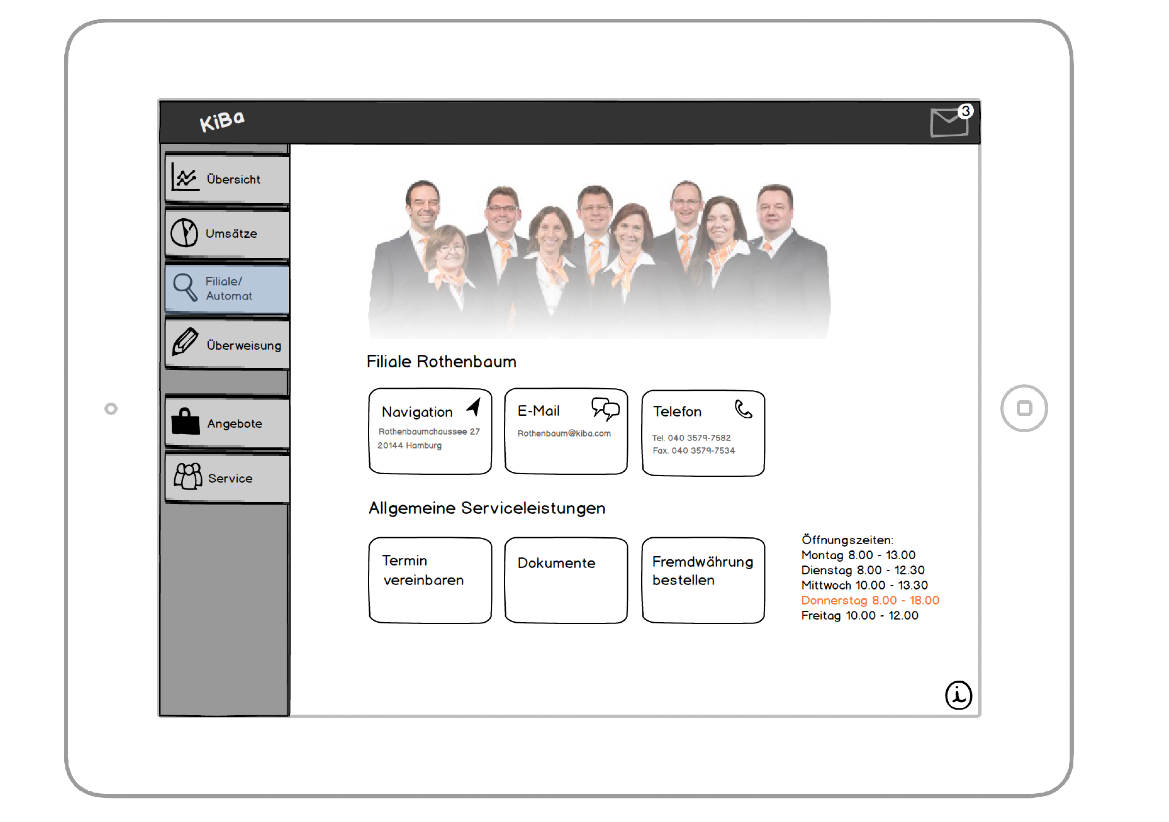
\includegraphics[scale=.52]{Pictures/MockupBranch}\\
	\includegraphics[scale=.52]{Pictures/MockupTransition}
	\caption{Mockup des Dashboards, der Filial-Seite und der Überweisung}
\end{figure}

	Die Elemente in der Detail-View sind asymmetrisch angeordet mit einer Gewichtung oben links und unten rechts. So erreichen wir eine diagonale Balance, die optimal für den optischen Fluss ist.

\subsection{Prototyp}
	Allgemein haben wir uns beim Design des User-Interface an den Guidelines von IOS7 orientiert. In diesem Zusammenhang haben wir uns mit den wichtigsten Grundsätzen laut Apple „Deference“, „Clarity“ und „Depth“ beschäftigt, um diese auf unser User-Interface zu übertragen. 
	
	„Deference“ haben wir bewirkt, indem wir den Fokus auf die Wahrnehmung von Inhalten gelegt haben und versucht haben, UI-Elemente, die in Konflikt mit dem Inhalt stehen, wegzulassen. Uns war es wichtig, das User-Interface möglichst funktional zu gestalten, was auch im Sinne von „Clarity“ ist. Daher haben wir eine möglichst selbsterklärende Ikonographie gewählt und auf eine unnötige Farbenvielfalt verzichtet. Den Guidelines entsprechend haben wir die Icons mindestens in der Größe 44 $\times$ 44 pts dimensioniert. Andernfalls wird es schwierig, ein Icon mit dem Finger zu treffen. Außerdem gibt es zu jedem Icon 2 Versionen, damit auf einem Retina iPad die hohe Auflösung ausgenutzt werden kann. Mit iOS7 setzt Apple auf Flat-Design. Ganz im Sinne des Flat-Designs haben wir eine dünne serifenlose Typographie ausgewählt und mit kräftig Kontrasten gearbeitet statt Schlagschatten oder Gradienten.

	Aufgrund von leichten Konzeptänderungen während des Projekts haben wir manche Details im Prototypen anders als in den Mockups gestaltet.
	
	Beispielsweise gab uns Markus Foos den Tipp, dass Nutzer mehr interessiert sind an den Umsätzen als an dem aktuellen Kontostand. Das ist besonders der Fall bei denjenigen Leuten, deren Kontostand niedrig ist oder die sogar im Minus liegen.. \par

\begin{figure}[h]
	\centering
	\includegraphics[scale=.52]{Pictures/Logo}
	\caption{App-Icon mit Farbskala}
\end{figure}
\subsection{Logo \& Farbharmonie}
	Unsere ausgewählte Farbharmonie spiegelt die Werte einer modernen Bank wider. Mit den Farben wollen wir Sicherheit, Nachhaltigkeit und Seriosität vermitteln. Allerdings waren wir bei der Logogestaltung in dieser Hinsicht nicht ganz konsequent. Wir hatten an dieser Stelle die Diskussion, ob wir uns nicht für ein anderes Logo entscheiden sollten. Mit dem KiBa-Glas im Logo haben wir uns dann darauf geeinigt, als Studenten ein wenig Humor zuzulassen. Im Zusammenspiel mit dem recht nüchternen Design wirkt das Logo auflockernd.

\subsection{UI-Elemete}
	Grundsätzlich haben wir mit den Standard-View-Elementen von iOS7 gearbeitet. Allerdings haben wir in machen Fällen auf ein Custom-Element zurückgegriffen und dieses dann konsequent eingesetzt. Bei dem Standard-Text-Field störte uns etwa, dass der Hint-Text bei der Eingabe verschwand und so die Eingabe gelöscht werden musste, um diesen wieder zu sehen. Man stelle sich vor, man möchte ein Überweisungsformular ausfüllen und während der Eingabe eines Feldes ist man sich nicht mehr sicher, wofür dieses steht. 

	Daher entschieden wir uns für eine Eigenlösung, die den Vorteil hat, dass der Hint-Text bei erfolgter Eingabe nach oben rückt und auf diese Weise sichtbar bleibt. 

\subsection{UX Inspektion \& Test}
	Wöchentlich hatten wir im Plenum die Möglichkeit, unseren Stand der App vorzustellen. Hier konnten in einer anschließenden Diskussion Unklarheiten im Konzept und Design angesprochen werden. Da sich im Plenum unter Anderem Dr. Kindsmüller befand, konnten wir von dem Wissen eines erfahrenen UX-Experten profitieren. Beispielsweise deckte er auf, dass wir eine Geste nicht erwartungskonform verwendeten. Bei der Scheck-Überweisung wollten wir anfangs mit der Wischgeste nach unten die Überweisung abschicken. Allerdings wird diese Wischgeste normalerweise als „Pull-to-refresh“-Geste verwendet. Daher war hier die Affordanz (Angebotscharakter) nicht gegeben. Um Verwirrung beim potentiellen Nutzer zu vermeiden, haben wir die Geste durch einen einfachen Button zum Abschicken der Überweisung ersetzt und die Animation entsprechend angepasst.

	Zwischendurch haben wir auch Kommilitonen die KiBa-App testen lassen. Wir stellten bei diesen kleinen Usability-Tests fest, dass das Konzept und der Sinn hinter der Authentifizierung nicht ganz verständlich war. Daher entschieden wir uns einen Comic zu erstellen, der die Kernschritte und Vorteile explizit erklärt. Auch ging aus der App nicht hervor, bei welchen Funktionen die Authentifizierung eine Rolle spielt. Diesen Mangel behoben wir, indem wir die Funktionen, welche erst nach der Authentifizierung verwendbar sind, mit einem Schloss-Icon markierten.
	
	Im Schlusssprint hatten wir die Möglichkeit, mit Herrn Kindsmüller jede View zu inspizieren, um auch die kleinen Interaktionsmängel aufzudecken. Beim Comic, der das Authentifizierungsverfahren erklärt, war beispielsweise der „Vorteil genießen“- Button für Nutzer nicht auffordernd genug. Dieses Problem der Salienz lösten wir durch eine leichte Animation. Des Weiteren wurde bei dem Kreditrechner nicht klar, dass individuelle Konditionen beim Berechnen eine Rolle spielen. Dr. Kindsmüller schlug uns vor, persönliche Assoziationen zu verwenden, wie „Ihr  Kreditrechner“ oder „Johns Kreditrechner“.

	All diese Erfahrungen zeigten uns, wie wichtig es ist, Kritik von außen einzuholen. Da wir in der Gruppe viel Vorwissen hatten, erschienen uns Dinge eindeutig, die für spätere Nutzer nicht unbedingt eindeutig sind.
Sicherlich wäre besser gewesen, früher mit dem Testen anzufangen.

	Dadurch das wir mit High-Fidelity-Prototypen getestet haben, gab es hauptsächlich Feedback zu kleineren Details und das gesamte Konzept wurde nicht in Frage gestellt. Trotzdem haben wir viel hilfreiche Kritik bekommen und konnten auf diese Weise mögliche Abbruchstellen in der UI beseitigen.

\authoredSection{alex}{Vorgehen}
\subsection{Orientierungsphase}
	Zu Beginn des Vorgehens standen Ideenfindung, Konzeption, Lernprozesse und das Finden eines gemeinsamen Arbeitsrhythmusses im Vordergrund. Eine erste grobe Orientierung, welche Aufgabenteile die einzelnen Beteiligten der Gruppe im Verlauf annehmen würden, ergab sich nach der „Kick-Off“-Veranstaltung bei T-Systems. Die Kompetenzen des Teams wurden anschließend auf die Positionen des Entwicklers, Konzepters, Projektleiters und Beraters aufgeteilt. 
	
	Zum Zeitpunkt der Ideenfindung wurde das Vorgehen noch weniger zentral organisiert, als es später durch den Projektleiter realisiert werden sollte. Es galt zunächst herauszufinden, mit welchen konkreten Aufgaben man sich im weiteren Verlauf konfrontieren konnte. Um eine grundlegende Kommunikation zwischen den Teammitgliedern zu etablieren, wurde eine Facebook-Gruppe gegründet, die dazu diente Ideen festzuhalten, zu besprechen und Termine oder Aufgaben für kommende Treffen zu vereinbaren. Um die Ideen darüber hinaus geordnet aufzuschreiben und für alle Beteiligten abrufbar zu machen, wurde zusammen mit dem Coderepository ein Wiki bei Github angelegt, siehe Abbildung \ref{fig:WikiHome}. Das Wiki fand im Speziellen in dieser frühen Phase Verwendung.
	
\begin{figure}[h]
	\centering
	\includegraphics[width=6cm]{Pictures/wiki_home}
	\includegraphics[width=6cm]{Pictures/wiki-konzept}
	\caption{Wiki bei Github\label{fig:WikiHome}}
\end{figure}

	Neben der Formfindung von Konzepten diente das Wiki ebenfalls zum Festhalten von Code-Style Konventionen (NYTimes Objective-C-Style Guide) oder Workflows, wie etwa dem toolunterstützten Erstellen von Doxygen-kompatiblen Methodenkommentaren mit dem Xcodeplugin VVDocumenter\footnote{\url{https://github.com/onevcat/VVDocumenter-Xcode}}. Auf Basis des Letzterem ließe sich bei Bedarf aus den Kommentaren eine Dokumentation im html-Format generieren. 

	Einen der ersten Schritte im Arbeitsprozess nach Erstellung des Exposés konnten wir mit Hilfe einer Umfrage bezüglich der Kundenbedürfnisse, -erwartungen und -bedenken respektive des Genres der Applikation, sowie unserer spezifischen Vorstellung, sprich der möglichen Features des Endprodukts, erreichen. Im Rahmen der ersten internen Treffens des Teams und der Plenumsveranstaltungen konnten sich die Vorstellungen langsam konkretisieren. Deutlich wurde dabei, wie diese zu priorisieren sind und welche Einschränken (wie bspw. Sicherheitsaspekte, Wertigkeit des Features) an eine mögliche Umsetzung geknüpft sind. In diesem Prozess wurde das Konzept stetig auf die Rückmeldungen der Plena angepasst. Begleitet wurde das Vorgehen durch das Erstellen von Mockups, die bereits in diesem Stadium helfen konnten, Inhalte nicht zuletzt visuell zu vermitteln und zu besprechen. Die Verwendung von Mockups fand aber auch im weiteren stets Anwendung, um Skizzen für eine mögliche Visualierung zu erstellen, bevor diese final umgesetzt wurden.

	Besonderes Augenmerk lag in der frühen Phase bezogen auf das Konzept im Herausarbeiten eines Alleinstellungsmerkmals, durch das sich mit Hilfe der Applikation die Fililalbank von der Direktbank positiv abheben kann. Dieser Punkt markierte gewissermaßen bei unserem Team die Hürde, um mit der eigentlichen Umsetzung zu beginnen. Die Featureideen sortierten wir fortlaufend neu nach geschätzter Priorität. Im Wiki unterschieden wir dabei grundsätzlich zwischen „Major“ und „Minor“.  
	
	Mit den Major-Features sollten die Kernfunktionalitäten der Applikation beschrieben werden. Hierzu zählten unter anderem der Filialfinder, der individuell angepasste Kreditrechner, sowie später primär fokussiert der Self-Service. Features, welche die App in der Gesamtheit aufwerten sollten aber nicht zur Kernfunktionalität gehören, bildeten die Minor-Kategorie. Ein Beispiel hierfür ist die Überweisungsfunktion für Girokonten. Sie wird in diesem Kontext erwartet, stellt aber keine Möglichkeit zur Abgrenzung gegenüber ähnlichen Anwendungen dar. Sie trägt außerdem nicht direkt dazu bei, die übergeordnete Fragestellung den Kunden wieder mehr an die Filialbank zu binden, zu erfüllen. Im Rahmen der Priorisierung verdeutlichte sich des weiteren, welche Features später nicht umgesetzt würden. Ein Feature das aufgrund niedrig eingestufter Priorität nicht den Weg bis in das Endprodukts geschafft hat, ist bspw. der SEPA-Umrechner, der das zuvor bestehende Format in die neue Kodierung umrechnen sollte. 
	
	Ebenfalls gab ausgedehnte Überlegungen, ob die Software für iPad, iPhone oder sogar dual für beide Geräte entwickelt werden sollte. Wie bei den Features war es auch hier hilfreich, wenn auch nicht einfach, demokratisch über eine Entscheidung abzustimmen. Dies zog auch nach sich, dass das Kollektiv den Einzelnen teils entgegen seiner eigenen Überzeugung zu einer gemeinsamen Lösung drängte. 
	
	Da die Kernfrage der Kundenbindung an die Filialbank schwer zu beantworten war, kam die Fragestellung des Zielgeräts und der damit verbundenen Auswahl an Features nach einer zuvor vermeintlich finalen Entscheidung mehrmals auf. Schlussendlich fiel die Entscheidung auf das iPad, weil wir die Kernfeatures durch dieses besser abdeckt sahen und sich nach der Umfrage der Eindruck einstellte, dass Nutzer sicherheitskritische Anwendungen bevorzugt in Ruhe Zuhause statt unterwegs verwenden wollen. Der Entschluss, sich bei der Entwicklung auf ein Gerät zu fokussieren, wurde teamintern unter den Gesichtspunkten mangelnden Gewinns einer dualen Entwicklung und dem damit verbundenen zusätzlichen Aufwand entschieden.

\subsection{Umsetzungsphase}
	Nachdem das grundlegende Konzept ausgearbeitet war, konnten wir mit der konkreten Umsetzung beginnen. Infolgedessen musste sich das Team auf einen Satz von Tools einigen, mit denen die Entwicklungsaufgaben verwaltet, zugeteilt und festgehalten wurden. Initial fiel die Entscheidung auf eine Kombination von Google-Docs und Github-Issues/Milestones. In Github lassen sich sog. Issues definieren. Diese Issues stellen Aufgaben dar, die Mitgliedern des Teams zugewiesen werden. Einzelne Issues werden wiederum Zwischenzielen zugewiesen, den Milestones. Sind alle Issues bezüglich eines Milestones abgearbeitet, ist dieses erfüllt. Die Verwaltung und Verteilung der Aufgaben wurde von diesem Zeitpunkt an durch den Projektleiter zentral durchgeführt. Alle neu entstehenden Aufgaben wurden also immer in Absprache mit diesem in das Issuesystem eingefügt. Dies war für die Übersicht der kommenden Aufgaben, verbunden mit der Gewissheit, dass alle Mitglieder über den Fortschritt im Ganzen wie im Einzelnen den gleichen Informationsstand haben, eine echte Hilfe. Die in Github eingetragenen Issues wurden neben der Zuweisung an Personen mit Labels versehen, die zum einen die Priorität zum anderen, das Überthema der Aufgabe beschreiben. Hochprior wurde u. a. das Erstellen einer Basisarchitektur auf der im weiteren softwaretechnisch aufgebaut werden sollte, sowie das Beschreiben der vorkommenden Entitäten und der damit verbundenen Relationen eingestuft. 

	Während wir GitHub zum Zuteilen und Festhalten der Aufgaben einsetzten, konnte mit Google-Docs der zeitliche Aufwand dafür festgehalten werden. Pro Aufgabe wurde eine Zeile mit entsprechendem Titel angelegt. Falls vorhanden, ist in der Tabelle das korrespondierende GitHub-Issue mit Verlinkung eingetragen. Die den Aufgaben zugewiesenen Teammitglieder sind mit Initialen vermerkt. Aus der tatsächlich aufgewendeten Zeit multipliziert mit der Anzahl der zugeteilten Personen resultiert der kumulierte Aufwand. Die Vorstellung der zu erledigenden Arbeiten war zu diesem Zeitpunkt allerdings meist unvollständig konkretisiert. Davon abgesehen gab es keine Vorerfahrungen bezüglich des iOS-Frameworks. Entsprechend mussten wir davon ausgehen, dass Aufwandsschätzungen zu Beginn nur bedingt hilfreich sein konnten. Trotzdem war dies als Vorlauf evtl. wichtig, um im  weiteren Verlauf ein gutes gemeinsames Verständnis für die Dokumentation und Verwaltung des Arbeitsaufwands zu entwickeln und zu präzisieren. 

\begin{figure}[h]
	\centering
	\includegraphics[scale=.25]{Pictures/gdocs1} \\
	\includegraphics[scale=.25]{Pictures/gdocs2}
	\caption{Google Doc\label{fig:GDoc}}
\end{figure}

	Während der Anfangsphase etablierte sich im Team ein Arbeitsrhythmus mit zwei Terminen pro Woche, in denen jeweilig das Arbeitspensum eines Werktages oder darüber hinaus absolviert wurde.  Die zeitlichen Gegebenheiten mussten auf unsere Gruppe von Studenten mit je unterschiedlichen Stundenplänen abgestimmt werden. In voller Gruppenstärke war es, abgesehen von Ausnahmen, folglich kaum möglich, außerhalb der festen Projekttermine zusammenzukommen. Um in unseren Arbeitsabläufen dennoch Kontinuität herzustellen, haben wir die vereinbarten Termine entsprechend organisiert, dass mindestens die Hälfte der Gruppe anwesend sein konnte. Folglich wurden die Termine alternierend in unterschiedlichen Besetzungen durchgeführt. 

	Die frühen Teamtreffen waren neben den eigentlichen Aufgabenstellungen stark davon geprägt, sich mit Objective-C, dem iOS-Framework sowie der Entwicklungsumgebung vertraut zu machen. Vielleicht wurde auch infolge dessen zunächst primär eine technische Umsetzung unter Vernachlässigung visueller Aspekte versiert. Nach der Rückmeldung in einem der frühen Plenumstermine, dass visuelle Gestaltung der technischen zeitlich nicht nachsteht und parallel dazu entwickelt werden sollte, wurde die Arbeitsweise dahingehend umgestellt. Technische und visuelle Gestaltung wurden von diesem Zeitpunkt an gleichzeitig entwickelt. 

\subsection{Vorgehensweise nach Scrum}
	Im Anschluss an die Scrum-Zertifizierung wurden Arbeitsabläufe und Positionierung der Mitglieder im Team erneut reflektiert, um einen Scrum-Prozess mit den entsprechenden Rollen zu realisieren. Korrespondierend zu den zuvor zugewiesenen Positionen des Entwicklers, Projektleiters, Beraters und Konzepters wurde nach Äquivalenten in der Scrum-Terminologie gesucht. Entwickler und Konzepter wurden der Gruppe des Development Teams zugeteilt. Während beim Berater eine Analogie zum Scrum Master gebildet wurde, lag es nahe, den Projektleiter dem Product Owner zuzuordnen. 

	Bereits vor der Zertifizierung hatte sich durch den Scrum Master die Praxis eines Daily Scrums eingestellt. Das Daily Scrum Meeting wurde immer zu Beginn jedes Treffens umgesetzt. Dies brachte den positiven Effekt mit sich, dass trotz alternierender Besetzungen sich alle Mitglieder zu Arbeitsbeginn über den aktuellsten Stand ausgetauscht hatten. Der Product Owner zuvor Projektleiter verwaltete weiterhin wie zuvor beschrieben zentral das Aufgabenmanagement. 
Problematisch erwies sich die zuvor getroffene Toolauswahl zur Organisation der Aufgaben unter den Gesichtspunkten von Scrum. Primär fehlte es den Tools an Möglichkeiten der Idee des iterativen Sprints gerecht zu werden. Infolgedessen stellte das Team die gesamte Toolchain zur Verteilung der Aufgaben und deren Aufwandsmessung um. Die Wahl fiel auf das Tracking-Tool PivotalTracker, in welchem die Terminologie Scrums mit Sprint-Backlog, Sprint-Velocity, „Done“- Status, usw. vertreten war. Die zuvor erstellten Issues und Aufwandseinschätzungen der noch offenen Aufgaben wurden komplett in die neue Umgebung übertragen.

\begin{figure}[h]
	\centering
	\includegraphics[scale=.25]{Pictures/pivottracker-overview}
	\caption{Stories bei PivotalTracker\label{fig:Pivottracker}}
\end{figure}

	Als Iterationsdauer legten wir einen Zeitrahmen von zwei Wochen fest. Diese Dauer erschien uns als sinnvoll; einerseits lang genug um, kleine oder mittelgroße Aufgaben innerhalb einer Iteration zu bewerkstelligen, anderseits nicht zu lang, um dynamisch auf geänderte Anforderungen reagieren zu können, ohne den Sprint-Backlog innerhalb eines Sprints modifizieren zu müssen. 
	
	Der Prozess des dynamischen Reagierens auf Kritik und sich damit ändernden Anforderungen vollzog sich über die gesamte Zeitspanne des Projekts. Das stetige Überdenken und Anpassen voriger Überlegungen und Ausarbeitungen stellte sich als eine der größten, wenn nicht als die größte Herausforderung des Projekts dar. Eine ständige Korrektur führt auch zum Verwerfen voriger Arbeit, woraus die Anforderung entsteht, sich stetig für neue Richtungswechsel zu motivieren.  

	Nach der Anfangsphase wurden die Aufwandsschätzungen präziser. Weiterhin war es zwar schwierig, genaue Schätzungen für einzelne Aufgaben vorzunehmen, insgesamt konnten wir aber trotz alledem auf Basis der sich ergebenden Sprint-Velocity ab dem letzten Drittel des Semesters eine sinnvolle Einschätzung über den verbleibenden Arbeitsaufwand und die dafür benötigte Zeit abgeben. Wie sich herausstellte, konnten wir diese Einschätzung auch einhalten. 

	Bezüglich der strengen Richtlinien von Scrum – entweder es wird auf voller Linie praktiziert oder aber das Vorgehensmodell ist nicht eingehalten und somit auch anders zu benennen – ist noch erwähnenswert, dass diese eigentlich vorsehen, dass das Development Team zu Beginn seiner Arbeit bereits alle notwendigen technischen Kompetenzen zur Umsetzung eines Projekts besitzt. Wir waren allerdings damit konfrontiert, selbstständig fortlaufend Wissen zu erarbeiten, das zur Bewältigung der Aufgaben notwendig war.

	 Neben den erwähnten Vorteilen des Tracking-Tools, respektive Struktur und Terminologie, ermöglichte uns die neue Umgebung das Verhältnis von bestehenden und noch zu erledigenden Aufgaben in Balkendiagrammen und Burndown-Charts zu visualisieren. Der Burndown-Chart bzw. Progress-Report über die gesamte zweite Hälfte der Projektdauer ergibt sich wie folgt:
	 
\begin{figure}[h]
	\centering
	\hspace{1.6cm}\includegraphics[width=.6\textwidth]{Pictures/burndown-compiled}
	\caption{Von PivotalTracker generiertes Burndown-Chart \label{fig:BurndownCompiled}}
\end{figure}

	Aus der Tendenz ist ersichtlich, dass die Sprint-Velocity unter Vernachlässigung der Ferienzeit stetig  bis zur Deadline zunahm.
\authoredSection{marco}{Ergebnis}
\subsection{Features}
\subsubsection{Dashboard}
\begin{figure}[h]
	\centering
  \includegraphics[scale=0.4]{Pictures/Dashboard}
	\caption{Dashboard}
	\label{fig1}
\end{figure}

Das Dashboard ist die zentrale Anlaufstelle der Applikation, dort haben wir einen Überblick über den Verlauf der Kontostände aller unserer Konten. In der Tabelle darunter haben wir die Möglichkeit alle Kontobewegungen nach zu verfolgen. 

%bild

\subsubsection{Filialfinder}
\begin{figure}[h]
	\centering
  \includegraphics[scale=0.4]{Pictures/filialfinder}
	\caption{Googlemaps mit Filialmarkierungen}
	\label{fig2}
\end{figure}

	Beim Filialfinder findet man eine Karte von Googlemaps mit Markierungen, welche die Standorte der einzelnen Filialen markieren. Mit einem Klick auf das Infosymbol gelangt man zur Filialseite auf der man die Öffnungszeiten nachschauen, aber auch eine Terminanfrage oder eine Sortenanfrage stellen kann. 

\subsubsection{Sortenanfrage}
%aktuelle Umrechnungskurse der europ. Zentralbank

\begin{figure}[h]
	\centering
  \includegraphics[scale=0.4]{Pictures/Sortenanfrage}
	\caption{Filialseite mit Sortenanfrage Pop-Over}
	\label{fig3}
\end{figure}

	Mit einem Klick auf Sortenanfrage bekommt der Nutzer ein Pop-Over zu sehen, in welchem er seine Wunschwährung auswählen kann die entsprechenden Umrechnungskurse werden intern direkt von der Europäischen Zentralbank bezogen. Hat man die Summe, welche umgetauscht werden soll eingegeben, so kann man die Anfrage stellen und bekommt eine Nachricht, ob die gewünschte Währung in der gewünschten Höhe bei der gewünschten Filiale verfügbar ist.

\subsubsection{Authentifizierung}
\begin{figure}[h]
    \centering
	\begin{tabular}{@{}cc@{}}
        	\includegraphics[width=1.5cm]{Pictures/notauth} &
    		\includegraphics[width=1.5cm]{Pictures/authed}
    \end{tabular}
	\caption{Die Authentifizierungsstati\label{fig4}}
\end{figure}

	Im oberen rechten Rand der Applikation ist ein kleines Symbol in Form eines Schildes zu sehen, dieses gibt den Authentifizierungsstatus zurück. Ein Schild mit einem Ausrufezeichen symbolisiert eine fehlende Authentifizierung, ein Haken eine gültige Authentifizierung.

	Solange das Gerät nicht authentifiziert ist, kann man einige Funktionen nicht benutzen, diese sind durch das Symbol mit dem geschlossenen Schloss gekennzeichnet.

	Unter dem Menüpunkt Authentifizierung findet man ein kleines Comic vor. Dieses erläutert wie der Nutzer sein Gerät bei seiner Filiale authentifizieren kann. Außerdem wird der Nutzer auf seine Vorteile aufmerksam gemacht.

\subsubsection{Überweisung}
	Unter dem Menüpunkt Überweisung findet man ein ganz gewöhnliches Überweisungsformular, die Überweisung muss man abschließend noch mit einem Tan bestätigen.

\subsubsection{Self-Service Station}
\begin{figure}[h]
	\centering
  \includegraphics[scale=0.4]{Pictures/SSverbunden}
	\caption{Self-Service Startseite. Die App ist verbunden.}
	\label{fig5}
\end{figure}

	Bei der Self-Service Station haben wir die Möglichkeit, sofern wir mit dem Stationsgerät verbunden sind, drei verschiedene Aktionen eigenständig durchzuführen. Eine Umbuchung, Kontoauszüge anschauen und drucken, sowie Bescheinigungen ansehen, ausfüllen und ausdrucken gegeben falls direkt abschicken.

	Jede Auswahlmöglichkeit hat eine kleine Tabelle mit Inhalten, die den User erwarten, wenn er auf den entsprechenden Button drückt.

\subsubsection{Bescheinigungen}
\begin{figure}[h]
	\centering
  \includegraphics[scale=0.4]{Pictures/Bescheinigungen}
	\caption{Die verschiedenen Dokumenttypen}
	\label{fig6}
\end{figure}

Bei den Bescheinigungen sehen wir verschiedene von der Bank zur Verfügung gestellten Dokumente die der Nutzer auswählen kann.

\subsubsection{Kontoauszüge}
\begin{figure}[h]
	\centering
  \includegraphics[scale=0.4]{Pictures/kontoauszuege}
	\caption{Übersicht der Kontoauszüge}
	\label{fig7}
\end{figure}

	Im Kontoauszugsbildschirm kann man Kontoaktivitäten in einem bestimmten Zeitraum drucken lassen. Somit kann man auch Kontoauszüge ausdrucken, welche man beispielsweise verloren hat und muss dies nicht beim Schalter beantragen.

\subsubsection{Umbuchungen}
\begin{figure}[h]
	\centering
  \includegraphics[scale=0.4]{Pictures/umbuchung}
	\caption{Eine Scheckgrafik als Formular für die Umbuchung}
	\label{fig8}
\end{figure}

	Im Umbuchungsbildschirm kann der Nutzer sowohl Ziel- als auch Quellkonto auswählen, zwischen denen der angegebene Betrag transferiert werden soll. Das ganze wird wird mit einem Button bestätigt.

\subsubsection{Finanzierungsrechner}
\begin{figure}[h]
	\centering
  \includegraphics[scale=0.4]{Pictures/finanzierung}
	\caption{Finanzierungsrechner mit individuellen Konditionen}
	\label{fig9}
\end{figure}

	Mit dem Finanzierungsrechner kann man sich Kreditkonditionen zusammenstellen. Die Werte der einzelnen Schieberegler werden aus dem Profil des Kundens von der Bank vorgegeben.

	Man kann danach auch wieder einen Beratungstermin vereinbaren um die Konditionen mit seinem Berater nochmal durchsprechen zu können, inwiefern die ausgewählten Konditionen empfehlenswert für den Kunden sind oder ob die Bank vielleicht noch bessere Sonderkonditionen anbieten kann.

\subsubsection{Mein Bereich}
%Nachrichtensystem
%mbereichneu.png

\begin{figure}[h]
	\centering
  \includegraphics[scale=0.4]{Pictures/mbereichneu}
	\caption{Ein minimalistischer Posteingang des Nutzers}
	\label{fig10}
\end{figure}

	Der Nutzer kann in seinem persönlichen Bereich Nachrichten der Bank empfangen und somit beispielsweise eine Bestätigung für seine Terminanfrage erhalten. Mit einem Klick auf die Zelle einer Nachricht bekommt man die entsprechende Nachricht in einer neuen Ansicht mit dem kompletten Nachrichtentext.

\subsection{Die Design-Highlights}
\begin{figure}[h]
	\centering
    %\begin{tabular}{@{}@{}}
	\caption{Eigenkreationen für das Design\label{fig11}}
\end{figure}

Um unserer Applikation in mancher Hinsicht besser auf unsere Bedürfnisse anzupassen haben wir uns bei einigen Designelementen über die Standardimplementierungen von Apple hinweggesetzt. Dennoch blieben die iOS-7 Richtlinien ein Qualitätsmaßstab für uns.

Wie in (A) zu sehen ist, bekam unser Schieberegler als kleine Erweiterung eine schwarze Sprechblase, welche den aktuellen Wert anzeigt. Dies ist unter anderem für die Bedienbarkeit implementiert worden, damit man beim Verschieben des Regler nicht immer auf die linke Seite schauen muss um den aktuellen Wert abzulesen.

Die mitgegebenen Textfelder von Apple haben in der Regel immer einen Text, welcher dem Nutzer einen Hinweis gibt was für ein Inhalt erwartet wird. Diese Umsetzung sieht oftmals unschön aus und nimmt viel Platz ein. Mit unserer Implementierung (B) verliert das Textfeld keine Funktionalität ist aber schlanker.

Die Standard Pop-Over lassen sich nur bedingt anpassen. So konnten wir die Farbe des Buttons nicht in unserem Farbton einfärben. Daher mussten wir auf eine Eigenimplementation (C) zurückgreifen um die Konsistenz zu wahren.

% Pop Over
% Sliderinfo
% mehr custom!!!!

\subsection{Herausforderungen}
	Mit zu den größten Herausforderungen war das Design der einzelnen Bildschirme. Das „Flat“-Design braucht ein gutes Händchen und kleine Details können schon zu Unstimmigkeiten führen. Gleichzeitig war uns bewusst, dass wir eine Bank repräsentieren und somit ein gewisses Maß an Seriosität erforderlich war. Gleichzeitig mussten wir die Usability für den Endnutzer gewährleisten. Wir mussten ein App-Design erschaffen, welches drei Stakeholder gleichzeitig zufriedenstellt.

%Die größte Herausforderung war aber ein sogenanntes "`Killer"'-Feature zu erschaffen. Nach unseren Erkenntnissen gibt es keine herausragende Eigenschaft der Filialbank, welche sie von Direktbanken unterscheidet. Vor allem nach der Finanzkrise ab 2007 ist das Vertrauen in Filialbanken stark gesunken, davor war die persönliche Beratung immer das Unterscheidungsmerkmal zu Direktbanken.
%Es bleibt nur noch die Finanzierung übrig, doch diese wird nur von einem Bruchteil der Kunden in Anspruch genommen. Berücksichtigt man noch die Anstrengungen der Direktbank auch eine persönliche Beratung per Telefonhotline anzubieten, indem der Kunde immer den gleichen Berater am Apparat hat, dann sieht man, dass selbst diese Lücke langsam aber sicher von den Direktbanken geschlossen wird.
%
%Wir als Entwickler konnten natürlich die Bank in ihrem Wesen nicht verändern, die Einführung von neuer Hardware mit der Self-Service Station war schon das Maximum an Veränderung die wir Einfordern konnten.

	Eine Herausforderung geht auch immer mit einer neuen Programmiersprache und deren Entwicklungsumgebung einher. Die ersten Wochen hatten wir eine relativ geringer Produktivität, weil wir uns auf diese Gegebenheiten erst einstellen mussten. Je weiter jedoch das Projekt voranschritt, desto sicherer fühlten wir uns in Objective-C und im Umgang mit Xcode.

	Während der Entwicklung stießen wir auch immer wieder auf Einschränkungen seitens Apple bezüglich der Standard GUI-Elemente. So konnten wir beispielsweise die Tint-Color eines Buttons im Pop-Over nicht ändern. Apple lässt es nicht zu. So mussten wir unser eigenes Pop-Over implementieren.

	Nichtsdestotrotz konnten wir alle größeren und kleineren Herausforderungen meistern und hatten nie das Gefühl vor einem unüberwindbaren Problem zu stehen.
\authoredSection{markus}{Architektur}
	Nachdem zunächst in diesem Bericht bereits Konzepte und Ergebnisse erläutert wurden gehen wir an dieser Stelle nun auf die Implementierung und technische Umsetzung der App ein. Im Fokus dabei steht die Architektur, die maßgeblich zum Ablauf der Entwicklung und zur Organisation der Kernkomponenten beiträgt.
	
	Unsere App soll den Kontakt zwischen einer Filialbank und seinen Kunden stärken. Da es sich bei KiBa lediglich um eine fiktive Bank handelt und die App auch anderen interessierten Banken vorgestellt werden soll, bietet es sich an, einen "Click-Dummy" zu entwickeln. Dieser soll sich bereits wie eine vollwertige Banking-App bedienen lassen, die jedoch an keine reale Bank, respektive deren Datenbank, angeschlossen ist. Aufgrund dieser Rahmenbedingungen, haben wir uns für die Architektur entschieden, die im Folgenden vorgestellt wird.

\subsection{Umsetzung des MVC-Ansatzes}
	Die Architektur muss uns dabei auf die Entwicklung der Kernfeatures fokussieren. Wenn nicht klar ist, welche Teile der Logik, der GUI oder anderer 

\subsection{Datenmodell}	
	Zur Modellbildung der App fiel unsere Entscheidung auf ein klassisches Entitäten-Be\-zieh\-ungs\-sys\-tem. Unser Weg zur Abstraktion einer Bank führt daher 
	über Klassen, die Modelle zu Objekten der realen Welt darstellen. Wie wir dabei vorgegangen sind ist im Entitäten-Relationen-Diagramm unseres Datenmodells in Abbildung \ref{fig:ERDiagram} zu sehen.
	
	\begin{figure}[h]
	\centering
	\scalebox{.57}{
	\begin{tikzpicture}[node distance=1.5cm, every edge/.style={link}]
		% User
		\node[entity] (User) {User};
		\node[attribute] (User1) [above=of User] {userId} edge (User);
		\node[attribute] (User2) [above right=of User] {forename} edge (User);
		\node[attribute] (User3) [above left=of User] {surname} edge (User);
		\node[attribute] (User4) [right=of User] {password} edge (User);
		\node[isa] (isa) [below=1cm of User] {is a} edge[->] (User);
		
		% Consultant
		\node[entity] (Consultant) [below left=1cm and 2cm of isa] {Consultant} edge[->] (isa);
		\node[attribute] (Consultant1) [left=1cm of Consultant] {phoneNumber} edge (Consultant);
		\node[attribute] (Consultant2) [above=1cm of Consultant] {image} edge (Consultant);
		\node[attribute] (Consultant3) [above left=1cm of Consultant] {businessPosition} edge (Consultant);
		
		% Customer
		\node[entity] (Customer) [below right=1cm and 2cm of isa] {Customer} edge[->] (isa);
		\node[attribute] (Customer1) [above=of Customer] {authenticated} edge (Customer);
		
		% Address
		\node[relationship] (livesAt) [below left=of Customer] {lives at} edge node[cty] {1} (Customer);
		\node[entity] (Address) [below left=of livesAt] {Address} edge node[cty] {1} (livesAt);
		\node[attribute] (Address1) [left=of Address] {street} edge (Address);
		\node[attribute] (Address2) [right=of Address] {houseNr} edge (Address);
		\node[attribute] (Address3) [below=of Address] {postalCode} edge (Address);
		\node[attribute] (Address4) [above=of Address] {city} edge (Address);
		\node[attribute] (Address5) [above left=of Address] {coordinates} edge (Address);
		
		% Branch
		\node[relationship] (Located) [below left=1cm and 1.5cm of Address] {location} edge node[cty] {1} (Address);
		\node[entity] (Branch) [below left=.5cm and 0.75cm of Located] {Branch} edge node[cty] {1} (Located);
		\node[attribute] (Branch1) [below=of Branch] {name} edge (Branch);
		\node[attribute] (Branch2) [above left=of Branch] {bic} edge (Branch);
		\node[attribute] (Branch3) [below left=of Branch] {openHours} edge (Branch);
		\node[attribute] (Branch4) [left=of Branch] {phoneNumber} edge (Branch);
		\node[relationship] (leads) [above=4cm of Branch] {leads} edge node[cty, swap] {1} (Branch) edge node[cty] {n} (Consultant);
		
		% Account
		\node[relationship] (owns) [below=2cm of Customer] {owns} edge node[cty] {n} (Customer);
		\node[entity] (Account) [below=2cm of owns] {Account} edge node[cty] {1} (owns);
		\node[attribute] (Acc1) [above left=.3cm and 1cm of Account] {balance} edge (Account);
		\node[attribute] (Acc2) [above right=-.2cm and 1cm of Account] {accountNr} edge (Account);
		\node[attribute] (Acc3) [below right=-.5cm and 1cm of Account] {description} edge (Account);
		\node[attribute] (Acc4) [below left=-.5cm and 1cm of Account] {overDraft} edge (Account);
		
		% Transaction
		\node[relationship] (recipient) [below left=1cm and .5cm of Account] {recipient} edge node[cty, swap] {n} (Account);
		\node[relationship] (sender) [below right=1cm and .5cm of Account] {sender} edge node[cty] {n} (Account);
		\node[entity] (Transaction) [below right=1cm and .5cm of recipient] {Transaction} edge node[cty, swap] {1} (recipient) edge node[cty] {1} (sender);
		\node[attribute] (Transaction1) [below=of Transaction] {amount} edge (Transaction);
		\node[attribute] (Transaction2) [right=of Transaction] {date} edge (Transaction);
		
		% OpenHour
		\node[relationship] (opens) [below right=.2cm and 1.5cm of Branch] {opens} edge node[cty] {n} (Branch);
		\node[entity] (OpenHour) [below right=.2cm and 1.5cm of opens] {OpenHour} edge node[cty] {1} (opens);
		\node[attribute] (OpenHour1) [below left=of OpenHour] {openingTime} edge (OpenHour);
		\node[attribute] (OpenHour2) [below=of OpenHour] {closingTime} edge (OpenHour);
		\node[attribute] (OpenHour3) [below right=of OpenHour] {weekDay} edge (OpenHour);
		
		% Message
		\node[relationship] (inbox) [below right=.5cm and .5cm of Customer] {inbox} edge node[cty] {n} (Customer);
		\node[entity] (Message) [below right=.5cm and .5cm of inbox] {Message} edge node[cty] {1} (inbox);
		\node[attribute] (Message1) [below right=of Message] {description} edge (Message);
		\node[attribute] (Message2) [below left=.8cm of Message] {content} edge (Message);
		\node[attribute] (Message3) [above right=of Message] {sender} edge (Message);
		\node[attribute] (Message4) [above=of Message] {date} edge (Message);
		\node[attribute] (Message5) [right=of Message] {msgId} edge (Message);
	\end{tikzpicture}
}
	\caption{Entitäten-Relationen-Diagramm \label{fig:ERDiagram}}
\end{figure}

\subsection{Sicherheitsaspekte}
	Ein wichtiger Aspekt, insbesondere im Hinblick auf den Umgang mit sensiblen Finanzdaten, ist die Sicherheit der App. Dabei ist es auch eine Aufgabe der Architektur, diese gewährleisten zu können. Im Folgenden erläutern wir die Schlüsse, die wir dementsprechend für die realistische Umsetzung zogen.
	
	Eine Fragestellung von essentieller Bedeutung für uns ist, was mit der App im Falle eines Diebstahls passieren würde. Da wir sowohl der Bank als auch dem Kunden gewährleisten müssen, dass ihre Daten sicher sind, haben wir das Risiko zu groß eingestuft, die Daten auf dem Gerät zu speichern. Deswegen liegen alle Informationen nur im Zwischenspeicher. Das hat für uns den Vorteil, dass beim Beenden der App alle Informationen verloren gehen, wenn der Kunde nicht mehr eingeloggt ist.
	
	Wichtig ist außerdem, dass alle Daten direkt übertragen werden. Wir stellen uns ein direktes Protokoll wie eine \acs{REST}-Schnittstelle oder ein \acs{SOAP}-Verfahren zum Austausch der Informationen zwischen App und Server der Bank vor.
	
	Insbesondere letzter Punkt kann es erforderlich machen, dass die Datenquelle anpassbar sein muss. Eine Möglichkeit, das zu realisieren, erläutern wir im nächsten Abschnitt.

\subsection{Dependency Injection}
	Eine zentrale Anforderung der App-Architektur für uns ist außerdem das Austauschen von einzelnen Kernkomponenten, wie etwa die Datenschicht. Denn hierdurch kann aus dem Click-Dummy eine vollwertige Banking-App erschaffen werden können, ohne große Änderungen am Code vornehmen zu müssen. Sie muss uns den Eindruck nehmen, an eine echte Bank gebunden zu sein.
	
	Daher ist für uns Dependency Injection als Entwicklungsmuster die Lösung dieses Problems. Wir haben es in einer reduzierter Form selber versucht zu implementieren. Dabei wird an einer zentralen Stelle im Quelltext, nämlich im \emph{Bootstrapping}, in den \texttt{KBADependencyInjector} registriert, welche konkrete Implementierung einer Abhängigkeit in der Anwendung verwendet werden soll. Beim \texttt{KBADependencyInjector} handelt es sich dabei nur um einen einfachen Schlüssel-Wert-Speicher. Der Bootstrapping-Prozess ist im Programmausdruck \ref{lst:Bootstrapping} wiedergegeben.
	
	\lstinputlisting[label={lst:Bootstrapping}, caption={Der Bootstrapping-Vorgang}]{Listings/Bootstrapping}
	
	Wie man sehen kann, besitzt jedes \ac{DAO} ein Protocol, welches auf zwei Arten instanziiert werden kann. Dadurch erreichen wir, dass ein Programm auf verschiedene Art und Weise ausführbar ist.
	
	Ein weiterer Vorteil dieser Abstraktion ist die Testbarkeit der App. Dadurch, dass im Click-Dummy feste Daten hinterlegt sind, kann man sich zum Testen der App verschiedene Fälle erzeugen, die einfach in den jeweiligen \texttt{DummyDao}s benutzt werden.
	
	Darüber hinaus erlaubt uns dieses Verfahren auch die erleichterte Austauschbarkeit einzelner Komponenten. Wenn man dieses Verfahren auf andere Funktionen der App anwendet, insbesondere dann, wenn benutzerspezifische Elemente erforderlich sind, so ist es schnell möglich, eine White-Label-App zu erzeugen. Das heißt also wir können eine App schaffen, die auf verschiedene Kunden zugemünzt werden kann. Dies hat für unseren Kunden den Vorteil, ihre App unter viele Kunden bringen zu können.
	
	Wir haben festgestellt, dass sich das frühe Auseinandersetzen mit seiner Softwarearchitektur eine gute Entscheidung ist. Durch die Implementierung unserer eigenen Dependency Injection und der zentralen Regelung von Abhängigkeiten an einem Ort haben wir eine dynamische und nachhaltige Methode geschaffen, unsere App sukzessive erweitern zu können.
\authoredSection{corny}{Toolchain}
Im Rahmen unseres Projekts wurde uns schnell klar, dass wir auf viele Tools angewiesen sein würden. So musste unser Quelltext versioniert, die grobe Struktur und Views festgehalten und Aufgabenpakete erstellt und koordiniert werden. Darüber hinaus war uns auch Design und Qualität wichtig. Auf unsere Erfahrungen in diesem Zusammenhang gehen wir im folgenden Abschnitt ein.

\subsection{Versionsverwaltung und Informationsaustausch}
	Um kollaborativ an einer Software zu arbeiten ist es selbstverständlich erforderlich, mit Quelltextversionierung zu arbeiten. Da bei uns Team-Mitgliedern die Erfahrung mit Git\footnote{\url{http://git-scm.com/}, Abruf am 23.02.2014 um 17:55 Uhr.} aus dem Universitäts- und Arbeitsumfeld am größten war, viel unsere Wahl für ein \acs{VCS} darauf.
	
	Entscheidend dabei war auch der größere Komfort gegenüber Subversion. Einerseits ist die operative Geschwindigkeit von Git deutlich schneller\footnote{\url{http://biz30.timedoctor.com/git-mecurial-and-cvs-comparison-of-svn-software/}, Abruf am 23.02.2014 um 18:05 Uhr.}, sorgt also im Team für eine Produktivitätssteigerung. Dieser Punkt ist in sofern für und von Relevanz, als dass auch wir ein Problem mit größeren Dateien, wie den XIB-Views, hatten. Auf der anderen Seite erlaubt Git durch sein verteiltes System Branches pro Anwender zu führen, wodurch auch ermöglicht wird, Commits  unabhängig vom Internet zu publizieren. 

\begin{figure}[h]
	\centering
	\includegraphics[scale=.25]{Pictures/GitHubOverview}
	\caption{Repository-Hosting bei GitHub \label{fig:GitHubOverview}}
\end{figure}
	
	Darüber hinaus schuf Git auch die Möglichkeit, die eng verwandte Plattform „GitHub“\footnote{\url{https://github.com/}, Abruf am 23.02.2014 um 17:55 Uhr.} als Repository-Hoster zu verwenden. Dieser bietet über den für die Versionsverwaltung erforderlichen Speicherplatz hinaus auch eine sehr gute grafische Bedienoberfläche, wie sie in Abbildung \ref{fig:GitHubOverview} zu sehen ist.
	
	Ein weiteres nützliches Feature von GitHub für uns war außerdem das zuvor erwähnte Wiki, dargestellt in Abbildung \ref{fig:WikiHome}. Ein Wiki hatte für uns den Vorteil eines demokratischen Informationsaustauschs; jeder konnte seine Erfahrung mit anderen Projektmitgliedern teilen, sodass alle davon profitierten. Daher tauschten wir in ihm erste Feature-Ideen oder auch Kontaktdaten aller Mitglieder aus. Allerdings nutzten wir es darüber hinaus auch für das Festlegen eines Arbeitsablaufs mit Xcode, ins Besondere das Code Styling oder das Verwenden bestimmter Plugins.

\subsection{Issue-Tracking-System}
	Da uns freundlicherweise von C1 WPS die Möglichkeit gegeben wurde, eine Scrum-Zer\-ti\-fi\-zie\-rung zu erhalten, lag uns viel daran, den Scrum-Ansatz so gut es ging in unseren Projekt-Ablauf zu integrieren. Dementsprechend war für uns bei der Frage nach einer unterstützenden Software wichtig, inwiefern es Scrum-Iterationen unterstützt und erleichtert.
	
	Dazu verwendeten wir – nach ersten Versuchen mit GitHub-Issues – die Software PivotalTracker. Mit ihr können wir, wie in Abbildung \ref{fig:TrackerStories} dargestellt, einzelne Stories erstellen und überwachen. Ein großer Vorteil dabei war, dass Scrum-Iterationen automatisch von der Software generiert werden, berechnet durch unsere durchschnittliche Arbeitskraft (genannt „Velocity“)\footnote{\url{http://www.pivotaltracker.com/community/tracker-blog/velocity-matters}, Abruf 23.02.2014 um 18:00 Uhr.} und unseren Vorhersagen für den Aufwand einer Story angegeben durch Punkte.
	
\begin{figure}[h!]
	\centering
	\includegraphics[scale=.25]{Pictures/TrackerStories}
	\vspace{-.8cm}
	\caption{Stories in PivotalTracker\label{fig:TrackerStories}}
\end{figure}

	Zum anderen generiert PivotalTracker auch Burndown-Charts, welche für das Vorgehen während der Scrum-Iterationen unabdinglich sind. Denn so können wir am besten den Fortschritt unserer App messen und haben ein Monitoring für das Fortschreiten der Entwicklung unserer Features zu sehen ist.

\subsection{Konzept- und Designwerkzeuge}
Balsamiq
\begin{figure}
	\centering
	\includegraphics[scale=.3]{Pictures/BalsamiqEntwurf}
	\label{fig:BalsamiqEntwurf}
	\caption{Entwerfen mit Balsamiq}
\end{figure}

Adobe Illustrator/Photoshop
\begin{figure}
	\centering
	\includegraphics[scale=.3]{Pictures/IllustratorIcon}
	\label{fig:IllustratorIcon}
	\caption{Designen des KiBa-Icons mit Adobe Illustrator}
\end{figure}
\authoredSection{corny}{Qualitätssicherung}
\begin{itemize}
	\item Gestaltungs-/Entwicklungsprozess (Mock-ups $\to$ Design $\to$ GUI-Bau $\to$ Logik)
	\item Design und iOS7-Guidelines
	\item Weeklies
	\item Feature-Improvement nach Plenarveranstaltungen
	\item Ausblick auf Unit Tests
	\item Club Mate
\end{itemize}

\authoredSection{michael}{Fazit}

Das Projekt objektorientierte Softwareentwicklung hat für uns in gewisser Hinsicht eine Zäsur im Studium markiert. Bisherige Module oder Praktika legten den Fokus auf eine technisch möglichst saubere Implementierung, bei der im Zweifel das Interaktionsdesign oder der Funktionsumfang zurückgestellt wurden. Im Projekt wurde die Beherrschung objektorientierter Techniken bereits vorausgesetzt und erstmalig ein Software-Produkt entwickelt, das in seiner Gesamtheit auch industriellen Anforderungen genügen musste. 

Mehrere Teilnehmer unserer Gruppe hatten bereits ein erstes Maß an Arbeitserfahrung vorzuweisen, etwa als Werkstudent oder freiberuflicher Webentwickler. Trotzdem wurde in den ersten Wochen des Projekts deutlich, dass im Bezug auf die Arbeitsorganisation als Auftragnehmer eines Produktes noch Raum für Verbesserungen war. 

Dies galt insbesondere für den Umgang mit Designfragen und der Reihenfolge der Entwicklung. In einer Gruppe, die bis auf eine Ausnahme aus Informatikstudenten bestand, gingen wir zunächst in aus anderen Modulen vertrauter Manier vor. Um die Eigenheiten von iOS und Objective C kennenzulernen, unternahmen wir erste Gehversuche in Funktionen wie einer Überweisungsansicht, die für das Endprodukt sekundär waren. Ebenso behandelten wir in den ersten Überlegungen das Design noch etwas stiefmütterlich. Eine Mentalität, der im Informatikstudium nicht selten Vorschub geleistet wird, ließe sich auf die Aussage „Erst wird programmiert, dann das Design nachgeschoben“ reduzieren. Im Plenum wurde uns aufgezeigt, dass ein solcher Ansatz nicht nur weniger effizient ist, sondern auch das eigene Produkt schlechter dastehen lässt. 

Denn einerseits ist es in einem engen Zeitrahmen, der ohnehin eher auf die Entwicklung eines Prototyps abzielt, sinnvoller, sich voll und ganz auf die Funktionen zu konzentrieren, die Alleinstellungsmerkmale darstellen und den innovativen Kern des Konzepts bilden. Denn nur anhand dieser lässt sich ein Kunde von einem Produkt überzeugen. Zudem erfordert ein benutzerzentriertes Design, das erst nachträglich hinzugefügt wird, umständliche Änderungen an der Codebasis. Gleichzeitig können bereits wenige, minimalistische Designelemente in konsistenter Farbe und Anordnung einen enormen Unterschied in der Wahrnehmung der Produktqualität bedeuten.

Entsprechend haben wir unsere Arbeitsweise adjustiert und ein neues Verständnis von zeitgemäßer Softwareentwicklung gewonnen. Während innovative Funktionalität von technischer Seite weiter geboten ist, hat sich der Anspruch der Benutzer an die Benutzbarkeit stark gewandelt; Apps, die dies nicht berücksichtigen, haben auf einem derart umkämpften Markt wenig Erfolgsaussicht.


\newpage
\renewcommand{\currentAuthor}{kiba}

%===============================================================================
% Bibliography
%===============================================================================
\def\mybibname{Literaturverzeichnis}
\renewcommand\bibname{\mybibname}
\renewcommand\refname{\mybibname}
\nocite *
\bibliographystyle{dinat}
\bibliography{Literature}

\end{document}